 
% Para una visualizacion correcta, generar el PDF
% Ni el DVI ni el PS se visualizan bien

% Elegir el estilo que se desee, hay cientos en la red

\documentclass{beamer}
\usepackage{beamerthemeshadow}
\usepackage{verbatim}
\usepackage{pgfpages}
\usepackage[galician]{babel}
%\usepackage[spanish]{babel}
\usepackage[utf8]{inputenc}
%\usepackage[latin1]{inputenc}
\usepackage[spanish,linesnumbered,lined,boxed,commentsnumbered,noend]{algorithm2e}
\usepackage{pgf-pie}
\usepackage{eurosym}


\setcounter{tocdepth}{1}% Allow only \chapter in ToC
\setbeameroption{show notes on second screen}
\setbeamertemplate{headline}{}


\begin{document}
\title[Intelixencia Artificial aplicada a Videoxogos Top-Down]{Intelixencia Artificial aplicada a Videoxogos Top-Down en tempo real}
\subtitle{Grao en Enxeñaría Informática \\
Universidade de Santiago de Compostela}  
\author{Autor: Rubén Osorio López}
\institute{Titor: Manuel Mucientes Molina\\Cotitor: Pablo Rodrígez Mier}
\date{21 de xullo de 2017} 

\begin{frame}
\titlepage
\note{Esto é a defensa da memoria do traballo de fin de grado nombrado \textbf{Intelixencia Artificial aplicada a Videoxogos Top-Down en tempo real}, eu son o autor, Rubén Osorio López, e os tutores son Manuel Mucientes Molina e Pablo Rodrígez Mier}
\end{frame}

\begin{frame}
\frametitle{Táboa de contidos}\tableofcontents
\note{Durante esta presentación seguiremos unha estructura similar á memoria, centrándonos máis en algunhos aspectos concretos do proyecto que expliquen en que consistiu o traballo realizado.}
\end{frame} 



\section{Introdución} 

\begin{frame}
\frametitle{Introdución} 


	\begin{itemize}
		\item Proxecto que aborda a creación dun \textbf{videoxogo} con necesidades de \textbf{comportamento complexo} por parte do inimigo.
	\end{itemize} 

\begin{block}{Videoxogo}
	\textbf{Loita 1 contra 1}, \textbf{Top-Down} en \textbf{dúas dimensións}
\end{block}

\begin{block}{Axente}
Capaz de percibir e actuar sobre o \textbf{entorno competitivo} do videoxogo mediante \textbf{sensores} e \textbf{actuadores}
\end{block}
\note{
	
	\begin{footnotesize}
	De forma general, búscase a \textbf{creación dun videoxogo que requira un enemigo con comportamento complexo}. O axente que representará o enemigo necesita ser un \textbf{competidor capaz}, para o que se realizou unha \textbf{etapa de entrenamiento} na que obtivo a información que necesitaba.\\
	\bigskip
	Para definir o videojuego, \textbf{Loita 1 contra 1} significa que solamente dous perxonajes competirán entre eles contando ambos cas mismas capacidades, accióis posibles e atributos. \textbf{Top-Down} refierese ó plano picado utilizado para visualizar o combate. Por outra parte que sea en \textbf{dúas dimensióis} implica que todo o contido do videoxogo son imagenes planas dibujadas unha a unha, sin que existan modelos en tres dimensiois.\\
	\bigskip
	\textbf{Un axente} é aquilo capaz de percibir o entorno mediante \textbf{sensores} e actuar sobre o mismo en consecuencia mediante \textbf{actuadores}, ambos son proporcionados pola súa interface co videoxogo. Ademáis atoparase nun entorno competitivo o que implica que buscará maximizar o seu \textbf{rendimiento} mentres se minimiza o do contrincante.
	\end{footnotesize}


}
\end{frame}




\subsection{Obxectivos}
\begin{frame}
\frametitle{Obxectivos} 
\begin{itemize}
	\pause
	\item Implementación do videoxogo \pause
	\item Implementación do axente \pause
	\item Realizar o adestramento do axente \pause
	\item Obter datos sobre as capacidades do axente \pause
	\item Analizar os resultados obtidos
\end{itemize}
\note{
\begin{footnotesize}
	Os objetivos to proyecto son os siguientes:
	\begin{itemize}
		\item Implementación do videoxogo: Xa que necesitaremos unha \textbf{plataforma que nos permita que o axente e o xogador interactúen} seguindo unha serie de regras comunes para competir entre eles.
		\item Necesitarase ademáis \textbf{implementar o axente capaz} de desenvolverse correctamente durante a competición.
		\item O axente necesitará \textbf{obtener a información necesaria para logo comportarse adecuadamente} gracias ó aprendido durante a etapa de entrenamiento.
		\item \textbf{Obteránse datos sobre o rendemento do axente} contra outras implementacióis máis sencillas.
		\item \textbf{Ca información obtenida} durante todo o proyecto, e especialmente na etapa anterior, \textbf{realizarase un análisis que describa o comportamiento do axente} e o que se conseguiu.
\end{itemize}
\end{footnotesize}
}
\end{frame}


\section{Videoxogo baseado en axentes}

\subsection{Mecánicas}
\begin{frame}
\frametitle{Mecánicas}

\begin{block}{Movemento}
Movemento libre nunha habitación rectangular.
\end{block}

\begin{block}{Ataque}
Permítese atacar a zona que se atopa cada onde o personaxe está mirando.
\end{block}

\begin{block}{Defensa}
Posibilidade de defenderse dun ataque permitindo atacar se a defensa ten éxito
\end{block}

\note{
\begin{footnotesize}
	Para explicar ahora o funcionamiento do videoxogo, empezarase polas mecánicas principales que o compoñen:
\textbf{O Movimiento} é libre nunha habitación rectangular o que suma a complexidade de evitar situacióis nas que non se poida escapar do contrincante por estar ó lado dunha parede ou unha esquina. Ademáis a única maneira de mirar cara unha dirección é moverse cara ela.\\
\textbf{Como} solo se permite atacar a zona directamente enfrente do personaje \textbf{é importante ter en cuenta cada donde se está mirando}. Esto favorece unha \textbf{actitude agresiva} pois hai que moverse na dirección do enemigo antes de atacalo.\\
\textbf{Pódese} realizar unha maniobra defensiva de \textbf{alto riesgo e alta recompensa} que permite evitar un ataque. Se se evita con éxito poderase realizar un ataque propio pero se non serase vulnerable durante uns instantes.\\
\textbf{Os tres estilos principales} que permiten estas mecánicas serán agresivo, defensivo ou contraataque. Nunha situación similar a un \textit{pedra, papel, tixeiras} cada un deles gaña e perde contra ún dos outros dous eliminando así a posibilidade de adoptar \textbf{un comportamento único} que sexa óptimo en todos os casos.\\
\end{footnotesize}
}
\end{frame}


\subsection{Prototipo de Unity}
\begin{frame}
\frametitle{Prototipo de Unity}
Primeira implementación realizada con \textbf{Unity3D}, estándar de facto para videoxogos de este tamaño.
	\vspace{0.5cm}
\begin{alertblock}{Problemas de simulación}
	Imposibilidade de escalar o tempo sen romper o funcionamento do videoxogo.
\end{alertblock}
\note{
	Para a primeira implementación destas mecánicas realizouse un prototipo inicial o antes posible no coñecido motor \textbf{Unity3D}, que é considerado \textbf{estándar de facto} para proxectos fora de grandes estudios.\\
	Gracias a estratexia realizada para mitigar o \textbf{riesgo 9} fíxose que este se materializara nunha etapa inicial do proyecto evitando unha situación imposible de gestionar posteriormente.\\
	\textbf{Ensinar vídeo}: Veremos ahora un vídeo que mostra algúns destes problemas.\\
	\textbf{Descubriuse} que facer pasar o tempo máis rápido dentro fo videoxogo, pese a estár soportado polo motor, rompe o funcionamento de moitos elementos necesarios como as caixas de colisións que impiden que un personaxe se saia do mapa ou a funcionalidade que xestiona os ataques do personaxe. Nestas circunstancias é imposible realizar un entrenamento acelerado válido para o axente polo que a aplicación non sería útil.
}
\end{frame}


\subsection{Segunda aplicación}
\begin{frame}
\frametitle{Segunda aplicación}
Implementación de un motor desde cero en C++

\begin{figure}
	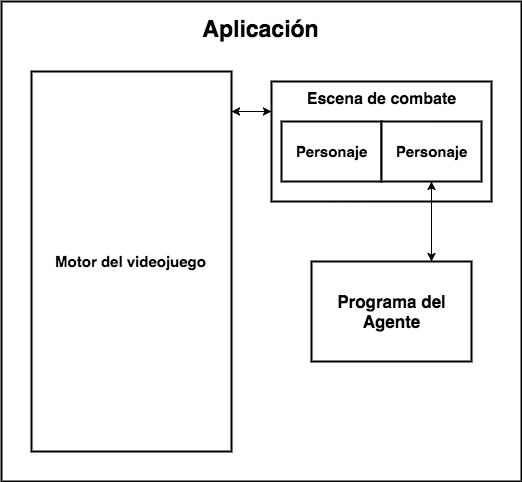
\includegraphics[scale=0.3]{../otros/otrasCapturas/block.png} 
\end{figure}

\note{
	A situación anterior fixo que surxira a necesidade de implementar a \textbf{aplicación dende cero}, para o cal se escolleu a linguaxe \textbf{C++} cunha serie de librerías a baixo nivel.\\
	\textbf{Na figura mostrada} podese ver como a aplicación completa estará composta por un motor que se encargará de todas as \textbf{funcionalidades genéricas}.\\
	Ademáis contarase cunha escena de combate con dous personajes, \textbf{un dos cuales está controlado} polo programa do axente, ainda que poderían ser ámbos.
}
\end{frame}

\subsection{Algoritmo}
\setlength{\algomargin}{0.11cm}
\begin{frame}
\frametitle{Algoritmo}
\begin{center}
	\scalebox{0.55}{
		\begin{minipage}{1.2\linewidth}
			\begin{algorithm}[H]
				\SetKwData{Action}{action}
				\SetKwData{LastAction}{selectedAction}
				\SetKwData{LastState}{lastState}
				\SetKwData{CurrentState}{currentState}
				\SetKwData{DeltaFitness}{deltaFitness}
				\SetKwData{StateActionData}{stateActionData}
				\SetKwData{RandomAction}{randomAction}
				\SetKwData{AllActions}{allPosibleActions}
				
				\SetKwFunction{GetRandomAction}{getRandomAction}
				\SetKwFunction{GetCurrentState}{getCurrentState}
				\SetKwFunction{RandomBet}{randomBetween}
				\SetKwFunction{CalculateFitness}{calculateFitness}
				\SetKwFunction{UpdateWith}{updateWith}
				\SetKwFunction{Insert}{insert}
				\SetKwFunction{Pick}{bestWeightedAction}
				
				\While{agent is running}{
					\LastState$\leftarrow$ \CurrentState\;
					\CurrentState$\leftarrow$ \GetCurrentState{}\;
					
					\DeltaFitness$\leftarrow$ \CalculateFitness{\CurrentState}$-$\CalculateFitness{\LastState}\;
					
					%Actualizamos el conocimiento del agente
					\uIf{\LastState$\in$ \StateActionData}{
						\StateActionData$.$\UpdateWith{\LastState,\LastAction,\DeltaFitness}\;
					}
					\Else{
						\StateActionData$.$\Insert{\LastState,\LastAction,\DeltaFitness}\;
					}
					
					
					%Seleccionamos la acción a escoger
					\uIf{\CurrentState$\in$ \StateActionData}{
						
						\uIf{\RandomBet{$0$,$1$}$<\epsilon$}{
							\LastAction$\leftarrow$ \RandomAction $\in$ \AllActions\;
						}
						\Else{
							\LastAction$\leftarrow$ \Action $\in$ \AllActions  $|$ \Pick{\StateActionData,\CurrentState} $=$ \Action  \;
						}
						
					}
					\Else{
						\LastAction$\leftarrow$ \RandomAction $\in$ \AllActions\;
					}
					
					
				}
				\label{algoritmo}
			\end{algorithm}
		\end{minipage}%
	}
\end{center}


\note{
	Pasarase ahora a explicar a grandes rasgos o funcionamento do algoritmo do axente. O mesmo é similar a unha implementación moi sencilla de \textit{Q-Learning}.\\
	Hasta a línea 8 da figura o que se fai e \textbf{obter o estado actual do combate} e calcular a \textbf{diferencia de utilidade} ou \textit{fitness} entre este e o anterior. Logo actualizarase a base de conocimiento do axente introducindo esta diferencia de fitness asociada a acción tomada para o último estado.\\
	\bigskip
	\textbf{A partir da liña 9} e hasta o final escollerase que acción se vai a levar a cabo cunha probabilidade proporcional ó fitnes que se espera de cada unha delas. Se o estado non se coñece escollerase unha acción aleatoria.\\
	\bigskip
	Ademáis, ainda que o estado se visitara, se un \textbf{valor aleatorio é menor} que certo \textbf{\textit{epsilon}} escollerase unha acción aleatoria de todas formas, facendo así que ainda que se coñeza ben o estado actual se permita explorar algunha das accións consideradas non optimas con máis frecuencia.
}

\end{frame}

\begin{frame}
\frametitle{\textit{Fitness}}


\begin{columns}
	\begin{column}{5cm}
\begin{center}
	\scalebox{0.5}{
		\begin{minipage}{1.6\linewidth}
			\begin{algorithm}[H]
					\SetKwData{Fitness}{fitness}
				
				\SetKwData{PlayerHealth}{playerHealth}
				\SetKwData{EnemyHealth}{enemyHealth}
				\SetKwData{Distance}{distance}
				\SetKwData{LookingAtEnemy}{lookingAtEnemy}
				\SetKwData{NoWallsNear}{noWallsNear}
				
				\SetKwFunction{GetRandomAction}{getRandomAction}
				\SetKwInOut{Input}{input}\SetKwInOut{Output}{output}
				\Input{\PlayerHealth, \EnemyHealth, \Distance, \LookingAtEnemy, \NoWallsNear}
				\Output{\Fitness}
				
				
				\Fitness$\leftarrow$ INITIAL\_FITNESS\_VALUE\;
				\Fitness$\leftarrow$ \Fitness$+ ($\PlayerHealth$*$ MY\_HEALTH\_MULTIPLIER$)$\;
				\Fitness$\leftarrow$ \Fitness$- ($\EnemyHealth$*$ ENEMY\_HEALTH\_MULTIPLIER$)$\;
				\Fitness$\leftarrow$ \Fitness$- ($\Distance$*$ DISTANCE\_MULTIPLIER$)$\;
				
				\If{\LookingAtEnemy}{
					\Fitness$\leftarrow$ \Fitness$+$ LOOKING\_BONUS\;
				}
				
				\If{\NoWallsNear}{
					\Fitness$\leftarrow$ \Fitness$+$ WALL\_BONUS\;
				}
				\label{algoritmo:fitness}
			\end{algorithm}
		\end{minipage}%
	}
\end{center}
	\end{column}
	\begin{column}{5cm}
		\scalebox{0.6}{
		\begin{minipage}{1.6\linewidth}
\begin{table}
	\begin{center}
		\begin{tabular}{|l|l|}
			\hline
			\textbf{Parámetro} & \textbf{Valor}\\
			
			\hline
			INITIAL\_FITNESS\_VALUE& 1000\\
			
			\hline
			MY\_HEALTH\_MULTIPLIER& 100\\
			
			\hline
			ENEMY\_HEALTH\_MULTIPLIER& 100\\
			
			\hline
			DISTANCE\_MULTIPLIER& 3\\
			
			\hline
			LOOKING\_BONUS& 200\\
			
			\hline
			WALL\_BONUS& 50\\
			
			\hline
		\end{tabular}
		\label{algoritmo:valores}
	\end{center}
\end{table}
\end{minipage}	
}
	\end{column}

\end{columns}


\note{
	Para obter o \textbf{fitness} simplemente se considerarán os valores de certas variables que representan o estado do combate. A saude do personaxe aumenta de forma \textbf{directamente proporcional} ó fitness mentres que a saude do inimigo e a distancia o fan de forma \textbf{inversamente proporcional}.\\
	\bigskip
	Ademáis proporcionaránse \textbf{dous bonus} por estár \textbf{mirando cara o enemigo} e por \textbf{evitar posicionarse ó lado dos muros} da escena.\\
	\bigskip
	Os valores usados para modificar o peso de cada unha das variables que se ven no cadro foron obtidos grazas a \textbf{coñecemento experto sobre o contexto do combate}. Céntranse en buscar un \textbf{comportamento agresivo e eficaz} por parte do personaxe que dea lugar a \textbf{pelexas dinámicas e entretenidas} para un xogador real.
}

\end{frame}


\subsection{Tipos de adestramento}
\begin{frame}
\frametitle{Tipos de adestramento} 

\begin{block}{Contra axente baseado en regras} % NEVER!!!!
	Pretende simular un aprendizaxe contra xogadores reais.
\end{block}

\begin{block}{Contra él mesmo}
	Buscando unha exploración mais extensa de estados que o axente baseado en regras non pode aportar.
\end{block}
\note{
	O algoritmo usarase de \textbf{dúas formas} para entrenar ó axente, \textbf{ben facendoo pelear contra outro axente basado en regras} simulando a un \textbf{xogador real} de forma moi sinxela. Ou ben \textbf{facendoo pelear contra él mismo} buscando a \textbf{exploración de estados} mui inusuales cuando se combate contra o axente basado en reglas.
}
\end{frame}



\section{Análise de requisitos}

\subsection{Casos de uso}
\begin{frame}
\frametitle{Casos de uso}
\begin{figure}[h]
	\vspace*{-0.8cm}
	\centerline{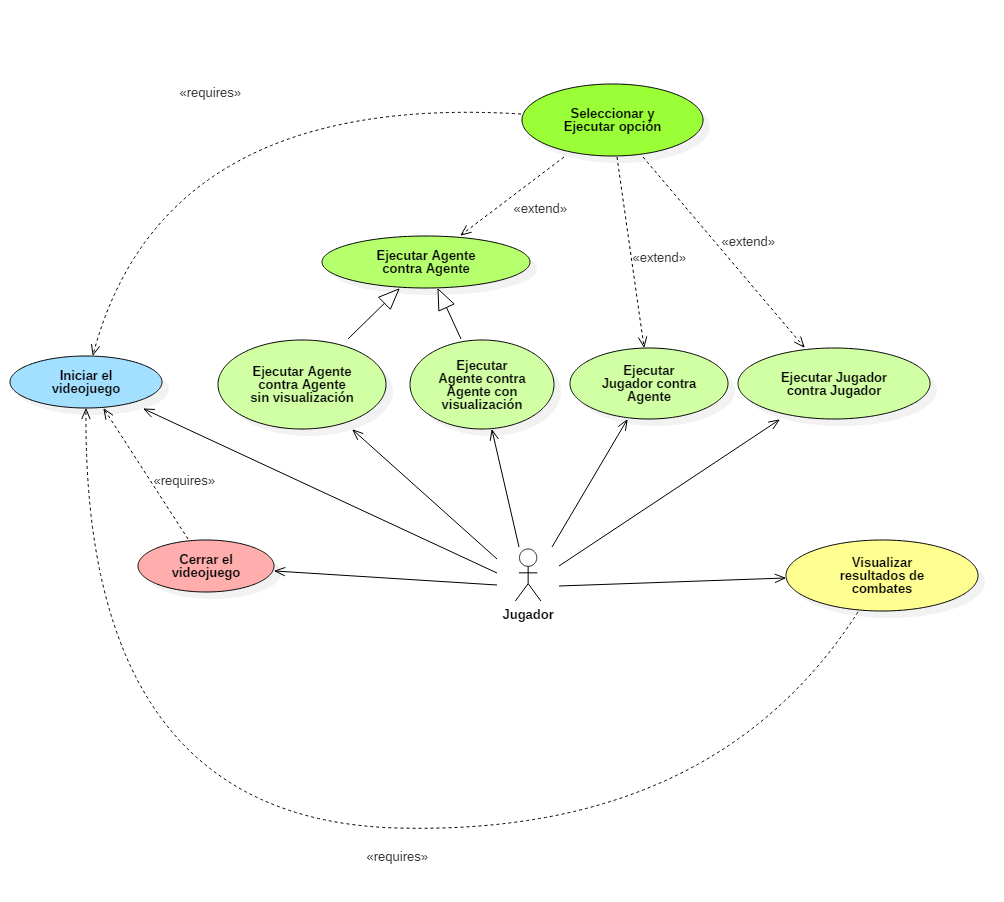
\includegraphics[width=10cm]{../diagramas/casosDeUsoCropped.png}}
	\label{casos_de_uso}
\end{figure}

\note{
	Entrando ahora dentro do bloque de analisis de requisitos, empezouse por identificar os diferentes casos de uso existentes no proxecto.\\
	\bigskip
	Empezando pola parte izquierda vemos en azul e rojo os casos de uso de \textbf{abrir e cerrar a aplicación}. En tonos \textbf{verdes} temos os casos de uso relacionados con seleccionar unha opción do menú e entrar na escena de combate apropiada, esta pode involucrar unha pelexa entre \textbf{dous axentes}, un \textbf{xogador real e un axente} ou \textbf{dous xogadores reales}.\\
	\bigskip
	Finalmente vemos en amarillo o caso de uso de visualizar os \textbf{resultados acumulados dos combates} o cual será necesario para ver o rendimiento do axente de forma sencilla especialmente cuando realiza combates sen que estes se mostren por pantalla.
	
}
\end{frame}

\subsection{Requisitos}
\begin{frame}
\frametitle{Requisitos}


\begin{columns}
	\begin{column}{5cm}
		
		
		\scalebox{0.75}{
		\begin{minipage}{2.0\linewidth}
		\begin{itemize}
			\item \textbf{RF-1/2/3}: Funcionalidades do menú
			\item \textbf{RF-4/15}: Consola con comandos/resultados
			\item \textbf{RF-5}: Saír da aplicación
			\item \textbf{RF-6}: Entrar na escena de combate
			\item \textbf{RF-7/8/9}: Moverse/Atacar/Defender
			\item \textbf{RF-10}: Gañar/Perder partida
			\item \textbf{RF-11}: Esgotar o tempo de combate
			\item \textbf{RF-12}: Volver ó menú
			\item \textbf{RF-13}: Visualizar combate entre axentes
			\item \textbf{RF-14}: Simular múltiples combates
		\end{itemize}
		\end{minipage}%
		}
	\end{column}
	\begin{column}{5cm}
			\scalebox{0.75}{
			\begin{minipage}{1.5\linewidth}
		\begin{itemize}
			\item \textbf{RNF-1}: Rendemento da aplicación
			\item \textbf{RNF-2}: \textbf{Velocidade das simulacións}
			\item \textbf{RNF-3}: Extensibilidade do motor
			\item \textbf{RNF-4}: Facilidade para depurar
			\item \textbf{RNF-5}: Aplicación autocontida
			\item \textbf{RNF-6}: Extensibilidade de escenas
			\item \textbf{RNF-7}: Documentación
			\item \textbf{RNF-8}: Usabilidade da interface
		\end{itemize}
	\end{minipage}%
}
	\end{column}
\end{columns}

\note{
	Dos anteriores casos de uso surxen unha serie de requisitos:\\
	\bigskip
	O primeiro grupo de requisitos funcionales relacionarase con moverse e seleccionar opcióis do menú e o siguiente cas funcionalidades da consola. Desde o requisito 5 hasta o 12 defínense funcionalidades relacionadas co combate e finalmente os dous últimos céntranse específicamente nos combates entre axentes.\\
	\bigskip
	Dentro do conxunto de requisitos non funcionales vense algunhos relacionados co \textbf{rendimiento da aplicación, a documentación ou usabilidade}. Destácase o \textbf{requisito non funcional 2} xa que é o que define formalmente a necesidade de poder simular peleas entre axentes de forma acelerada, o cual, como se viu anteriormente, tuvo un peso importante no proyecto.
}
\end{frame}

\section{Xestión do proxecto}

\subsection{Xestión de riscos}
\begin{frame}
\frametitle{Xestión de riscos}

\begin{block}{Identificación de riscos}
	Identificáronse e especificáronse un total de \textbf{10} riscos, destacándose o \textbf{RSK-1} (retraso na planificación), \textbf{RSK-2} (cambio de requisitos) e \textbf{RSK-9} (dificultade para realizar simulacións).
\end{block}
\bigskip
\begin{alertblock}{Acción correctiva AC-1}
	Xestionou a materialización do \textbf{RSK-9} e implicou implementar dende cero a aplicación do videoxogo sen facer uso dos motores dispoñibles.
\end{alertblock}

\note{
	Chegando á gestión de riesgos, identificáronse un total de 10, dos cuales destácanse pola súa probabilidade é impacto o \textbf{1} relacionado con retrasos na planificación, o \textbf{2} relacionado con cambios nos requisitos e o {9} relacionado con non poder realizar simulacións de combates.\\
	\bigskip
	A única acción correctiva que e levou a cabo é a asociada ó prototipo de Unity e á implementación da aplicación desde cero como xa se mencionou anteriormente.
}
\end{frame}


\subsection{Metodoloxía}
\begin{frame}
\frametitle{Metodoloxía}

\begin{block}{Contexto do proxecto}
\begin{itemize}
	\item Traballador único
	\item Duración relativamente corta
	\item Necesidade de avanzar rapidamente nas etapas iniciais
\end{itemize}
\end{block}
\bigskip
\begin{block}{Programación Extrema}
	\begin{itemize}
		\item Flexibilidade ante cambios
		\item Evitase utilizar demasiado tempo en tarefas de xestión
		\item Rápida iteración
		\item Reunións entre \textit{sprints}
	\end{itemize}
\end{block}

\note{
	A elección de metodología tuvo muito que ver cas circunstancias do proyecto. Neste caso \textbf{non era necesario dedicar muitos recursos a coordinar ós traballadores} xa que solo había un, a \textbf{duración} do proyecto foi relativamente corta \textbf{comparada con outros dentro da industria dos videoxogos} e necesítábase avanzar rápidamente para \textbf{rematar a aplicación o antes posible} é poder dedicar tempo ó axente.\\
	\bigskip
	Dentro das metodologías ágiles escolleuse \textbf{Programación Extrema} pola súa \textbf{flexibilidade ante os cambios que probablemente ocurrirían}. Ademáis non se dedica un \textbf{tempo excesivo a tareas de gestión que ralenticen o desenvolvemento do proyecto}. E os Sprints realizados entre as distintas reunións permiten que os \textbf{tutores axuden a detectar problemas} en ventás de tempo muy pequenas.
}
\end{frame}

\subsection{Planificación temporal}
\begin{frame}
\frametitle{Planificación temporal}

\begin{center}
\begin{tikzpicture}
	% squere, cloud
	\pie[sum=auto, after number={d}, cloud, radius = 2]{37/Videoxogo, 16/Axente, 3/Obtención de datos}
\end{tikzpicture}
\end{center}

\note{
	A planificación temporal final dividese tal e como se mostra nesta figura, pero os grupos de tareas que se levaron a cabo durante todo o proyecto como \textbf{documentación e reunións non están presentes}.\\
	\bigskip
	Vemos como o desarrollo do prototipo en Unity e da aplicación final teñen un peso muy importante na planificación con 37 días, o que deixóu unhos 16 días de traballo para a creación e entrenamiento do axente. Finalmente dedicáronse 3 días a obter datos sobre o rendimiento do mismo.
}
\end{frame}

\subsection{Xestión de custos}
\begin{frame}
\frametitle{Xestión de custos}

\begin{block}{Custos a incluír}
	\begin{itemize}
		\item Soldo do traballador: 3952.50 \euro
		\item Amortización do equipo de traballo: 194.90 \euro
		\item Impresión da memoria + CD: 100 \euro
		\item 10\% de custos indirectos: 424.74 \euro
	\end{itemize}
\end{block}

\bigskip

O que resulta nun custo final de \textbf{4672.14 \euro}


\note{
	De forma breve, mostrase aquí \textbf{qué elementos contribuiron} a aumentar o coste do proyecto dando lugar a  un importe final de \textbf{4672.14 \euro}. Débese destacar que todas as \textbf{ferramentas usadas eran ou ben libres ou versións de proba} polo que non implicaban un coste monetario.
}
\end{frame}

\section{Arquitectura}
\subsection{Arquitectura do sistema}
\begin{frame}
\frametitle{Subsistemas conectados}

\begin{figure}
	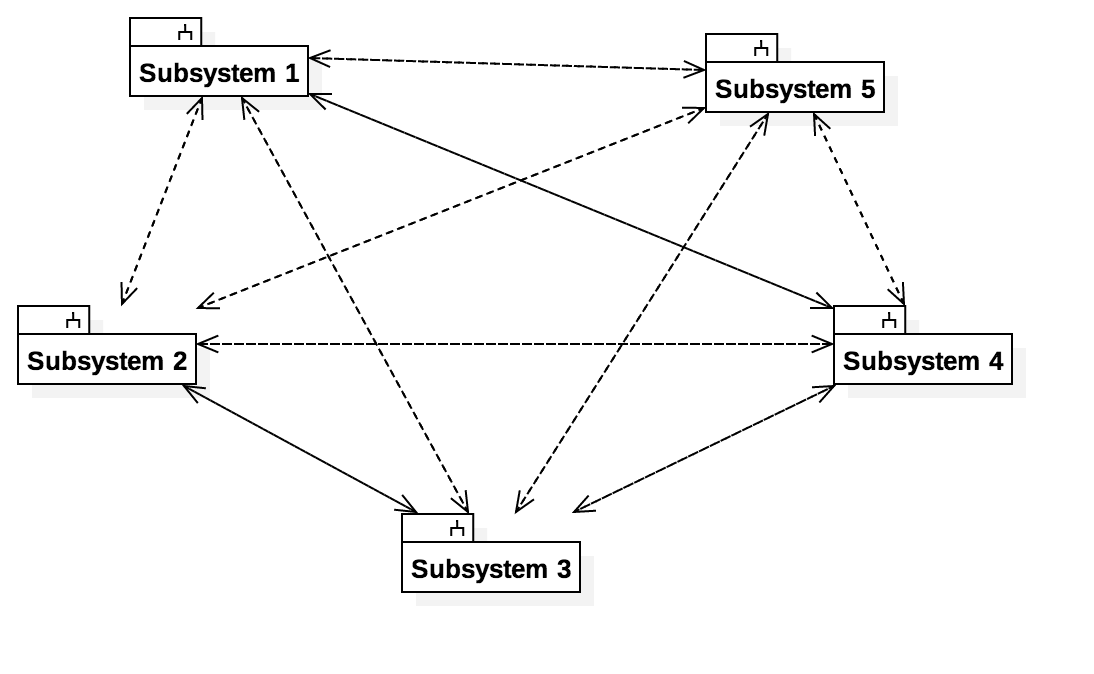
\includegraphics[width=10cm]{../otros/UML/png/arquitectura_mala.png}
	\label{dia:arquitectura_mala}
\end{figure}
\note{
 	A arquitectura da aplicación componse por unha serie de \textbf{subsistemas que necesitan conectarse unhos cos outros con moita frecuencia}. Na figura vemos como unha aproximación simple na que todos teñen referencias a todos pode levar a\textbf{ muitos problemas }orixinados por ter que cambiar calquera cousa en algún deles.
}
\end{frame}
\begin{frame}
\frametitle{Bus de mensaxes}
\begin{figure}
	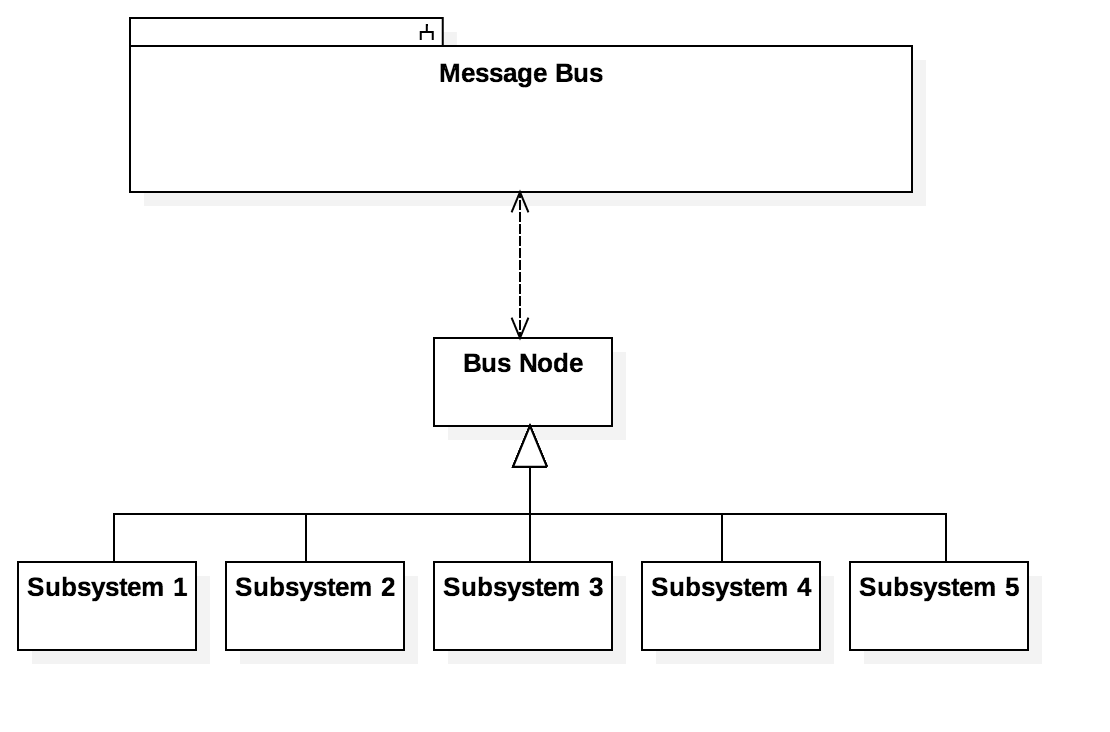
\includegraphics[width=10cm]{../otros/UML/png/actual_arquitecture.png}
	\label{dia:actual_arquitecture}
\end{figure}
\note{
	A solución diseñada foi crear un \textbf{bus de mensajes}. Nesta arquitectura todos os \textbf{subsistemas son un nodo} dese bus, podendo comunicarse con calquera dos outros subsistemas ou con todos á vez mediante o \textbf{envío de mensajes}, evitando referencias innecesarias. Nesta arquitectura cada subsistema elige como gestionar os mensajes que recibe.\\
	\bigskip
	A arquitectura terá un aspecto similar á siguiente:
}
\end{frame}
\begin{frame}
\frametitle{Arquitectura final}
\begin{figure}
	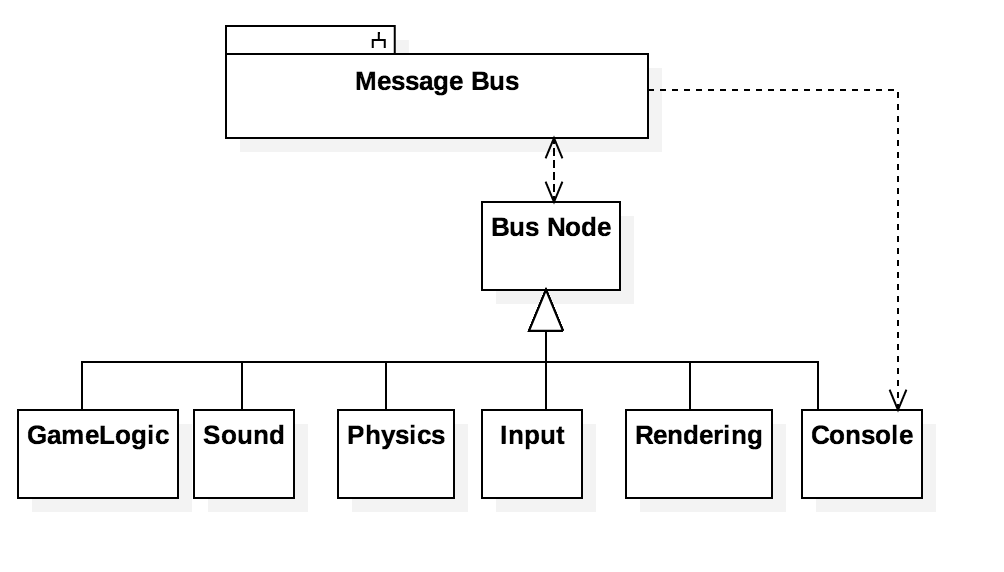
\includegraphics[width=10cm]{../otros/UML/png/final_arq.png}
	\label{dia:arquitectura_final}
\end{figure}
\note{
	Aquí vemos os diferentes subsistemas existentes así como unha \textbf{dependencia} do bus de mensajes ca co subsistema da \textbf{consola}. Esto permite que en tempo de ejecución se poida \textbf{visualizar} en calquera momento calquera mensaje relevante na ventá da propia aplicación ademáis de \textbf{introducir} \textbf{mensajes} co contido que se queira dentro do bus de mensajes.\\
	\bigskip
	Esto resultóu extremadamente útil xa que facilitóu moito o proceso de \textbf{debug} e axudou a unha \textbf{iteración muy rápida}.
}
\end{frame}



\section{Deseño}
% Agregar  o diagrama de clases do "GAME simplificado"
\begin{frame}
\frametitle{Diagrama de clases xeral}
\begin{figure}
	\vspace*{-1cm}
	\hspace*{-0.5cm}
	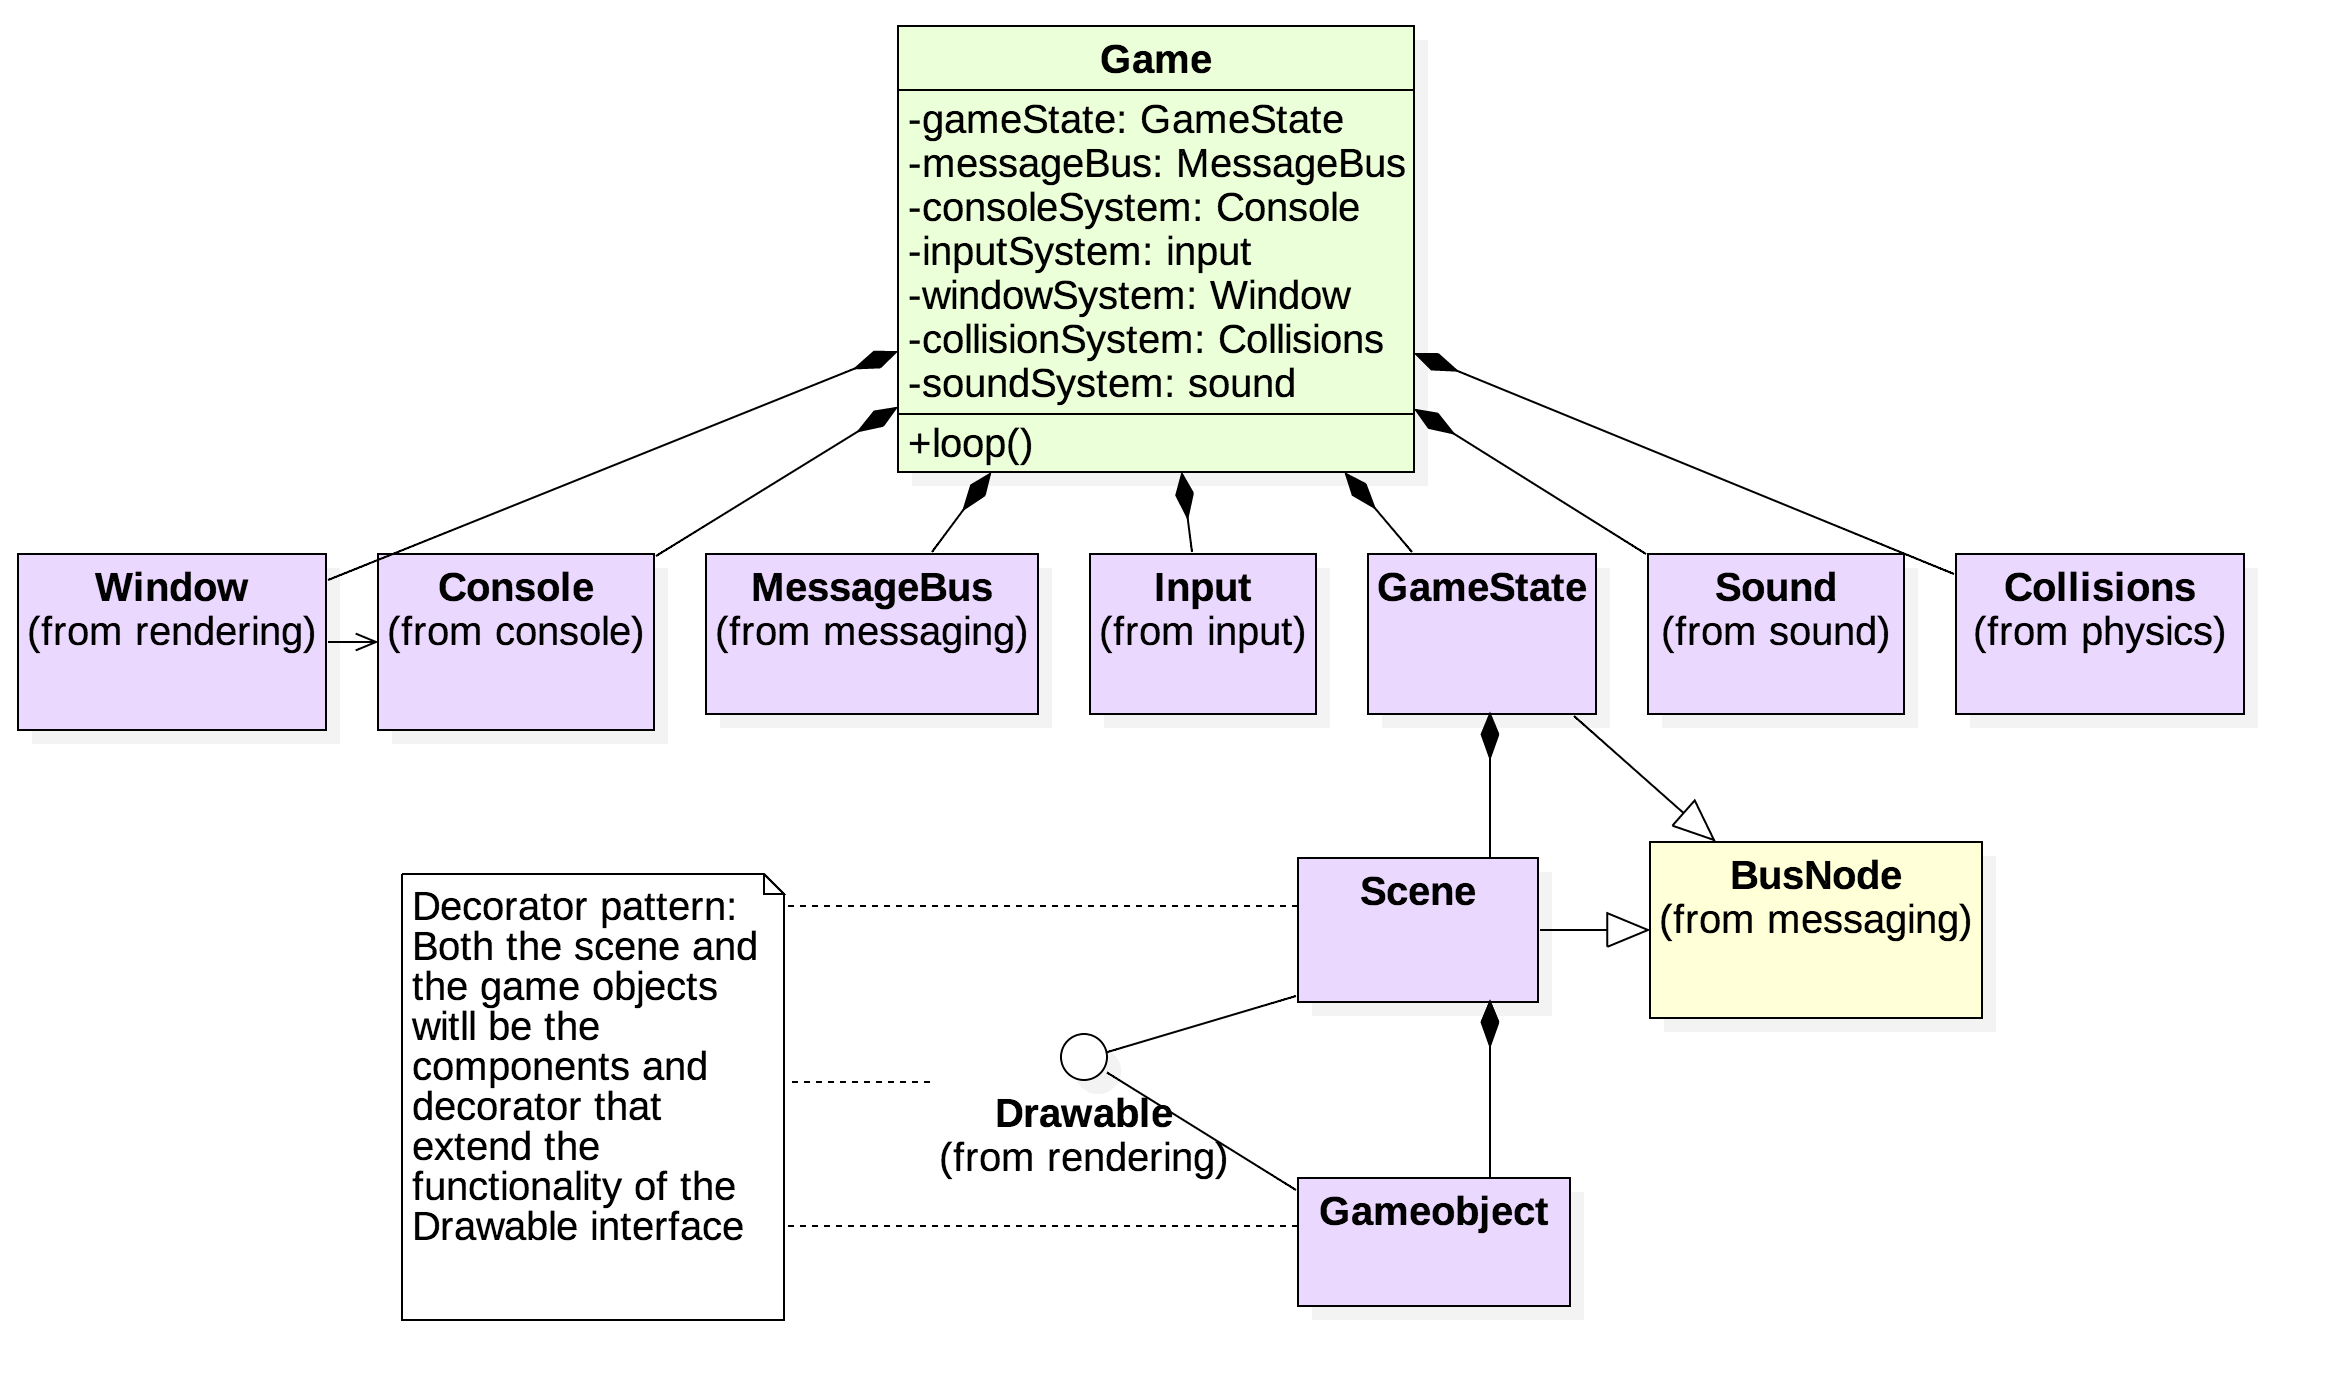
\includegraphics[width=12cm]{./diagramaDeClases_gamelogic_simple.png}
	\label{dia:clases}
\end{figure}
\note{
	No que respecta a diseño e implementación, para non entrar demasiado en materia, mostrase solamente o diagrama que representa a \textbf{clase principal de cada subsistema} e a clase \textit{\textbf{xogo}} que os contén e itera sobre eles.\\
	\bigskip
	Ademáis podese ver como se conta ca clase \textit{\textbf{scene}}, que representa calquera \textbf{escena} na que pode estár o videoxogo como un menú ou o combate. Esta clase contará cunha serie de \textit{\textbf{GameObjects}} que poderán ser calquera \textbf{entidade dinámica} no contexto do videoxogo como un personaje, unha barra de vída ou unha opción do menú. Esto permite muita \textbf{flexibilidade á hora de implementar} cada unha de estas entidades.
}
\end{frame}

\section{Validación e probas}
\subsection{Aplicación}
\begin{frame}
\frametitle{Validación e probas da aplicación}
\begin{block}{Probas unitarias}
	Unha ou mais probas por cada requisito tanto funcional como non funcional superadas na sua totalidade.
\end{block}

\begin{block}{Probas de integración}
	Comproban a integración entre subsistemas e do o axente ca aplicación.
\end{block}
\note{
	Chegando xa ó apartado de validación e probas, realizáronse unha serie de \textbf{probas unitarias} para os múltiples \textbf{requisitos funcionales ou non} do proxecto.\\
	\bigskip
	Ademáis levaronse a cabo probas de \textbf{integración} para comprobar o funcionamento dos \textbf{subsistemas conectados} e do \textbf{axente dentro da aplicación}.
}
\end{frame}
\subsection{Validación do Axente}
\begin{frame}
\frametitle{Comparativa de vitorias}

\begin{figure}[h]
	\centerline{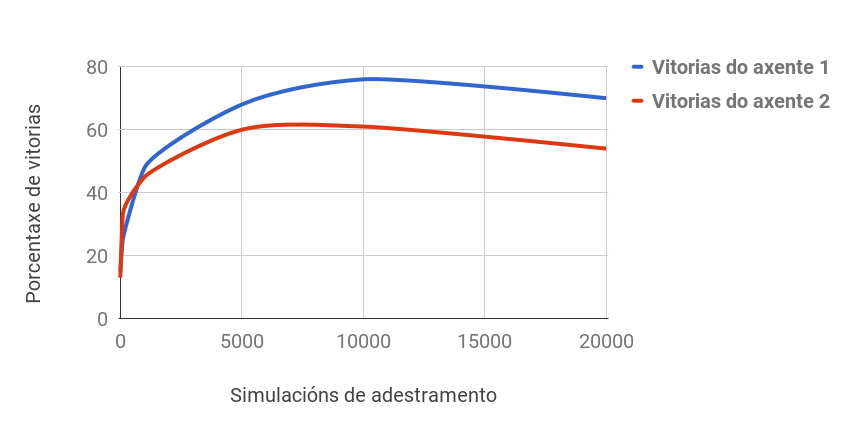
\includegraphics[width=11cm]{./graficos/vitorias.png}}
	\label{graf:victorias}
\end{figure}
\note{
	\begin{footnotesize}
	En relación á \textbf{validación do axente} realizase nesta figura un análisis que compara o rendemento do \textbf{axente 1} entrenado únicamente contra o personaxe basado en reglas contra o \textbf{axente 2} entrenado únicamente contra él mesmo.\\
	\bigskip
	Dado que para calcular o porcentaxe de victorias se realizaron \textbf{100 combates contra o personaxe basado en reglas}, obsérvase como o axente que entrenou contra él representado pola línea azul é significativamente mellor que o outro.\\
	\bigskip
	Tamén é interesante como o axente \textbf{2 gaña con moi poucas simulacións} debido a que está \textbf{aprendendo o doble de rápido} xa que os dous personajes están aprendendo á vez e combinando a información aprendida.\\
	\bigskip
	Finalmente hay que destacar como unha vez que se superan uns \textbf{10.000} combates se sufre de \textbf{\textit{overfitting} ou sobreaxuste}. Neste caso, pese a que o fitness dos estados siga aumentando co entrenamento, o mismo non ten por que estár \textbf{relacionado linealmente coa probabilidade de obter unha victoria}.
\end{footnotesize}
}
\end{frame}

\begin{frame}
\frametitle{Comparativa de estados visitados}
\begin{figure}[h]
	\centerline{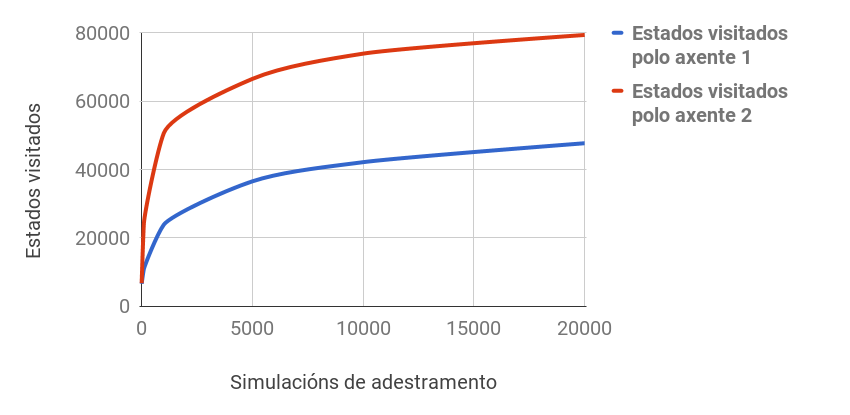
\includegraphics[width=11cm]{./graficos/estados.png}}
	\label{graf:estados}
\end{figure}

\note{
	Mui brevemente, nesta gráfica vemos como o axente que entrena contra él mesmo sí realiza unha \textbf{exploración de estados moito máis extensa} e dunha forma moito máis rápida polo que é menos probable que ó \textbf{combatir contra un xogador real }se atope en situaciois nas que non sepa como responder.\\
	\bigskip
	A partir de unhas 20.000 iteracióis o \textbf{aumento} de estados visitados \textbf{non compensa} o tempo necesario para seguir entrenando.
}
\end{frame}

\begin{frame}
\frametitle{Axente escollido}
Combinación de ámbolos dous métodos de adestramento.

\begin{block}{Contra o axente baseado en regras}
	Favorece un aprendizaxe moi rápido nas primeiras simulacións.
\end{block}

\begin{block}{Contra él mesmo}
	Aporta unha exploración de estados superior.
\end{block}
\note{
	Finalmente o axente escollido intenta \textbf{combinar o mellor dos dóus métodos de entrenamento}, empezando a aprender contra o axente basado en reglas para \textbf{aprender rápidamente a gañar partidas} e seguindo con combates contra él mismo para ter \textbf{acceso a unha grán cantidade de estados}.\\
	\bigskip
	Ahora mostrarase o comportamiento do axente en tempo real nun \textbf{combate contra un xogador humano}, que seréi eu. E despois describiranse dous comportamentos interesantes que aprendeu na etapa de entrenamento \textbf{ca axuda dun vídeo}.
}
\end{frame}


\section{Conclusións}

\subsection{Conclusións e leccións aprendidas}
\begin{frame}
\frametitle{Conclusións e leccións aprendidas}
\begin{block}{Logros do proxecto}
\begin{itemize}
	\item O comportamento, aspecto e rendemento da aplicación cumpriu as expectativas.
	\item O axente é capaz de competir contra outras implementacións e contra xogadores humanos.
\end{itemize}
\end{block}

\begin{block}{Leccións aprendidas}
	\begin{itemize}
		\item Importancia de ter en conta os posibles riscos do proxecto o antes posible.
		\item Utilidade de un deseño flexible previo á implementación.
		\item Calidade dos resultados de implementacións sinxelas de Intelixencia Artificial.
	\end{itemize}
\end{block}

\note{
	\begin{footnotesize}
	A modo de conclusión, considérase que a aplicación cumpliu as espectativas xa que o seu \textbf{rendemento é mellor do esperado}. Ademáis o \textbf{axente resultou ser muy capaz} incluso contra xogadores relativamente experimentados neste tipo de videoxogos e este en concreto.\\
	\bigskip
	Algunhas das \textbf{leccióis importantes} que se aprenderon temos:\\
	\textbf{A importancia de dedicar} un momento a considerar que pode \textbf{sair mal} en calquera proxecto para lidiar cos problemas antes de que sean demasiado importantes.\\
	\textbf{As facilidades} que proporciona seguir un \textbf{diseño flexible} e definido en vez de empezar a implementar directamente por considerar que non hay o tempo suficiente.\\
	\textbf{E que as técnicas intelixencia artificial}, incluso con implementacións tan sencillas como esta, son realmente \textbf{capaces} e os seus límites están máis alá do que nun primeiro momento se podería pensar.
	
		\end{footnotesize}
}

\end{frame}

\subsection{Posibles ampliacións}
\begin{frame}
\frametitle{Posibles ampliacións}
\begin{itemize}
	\item Melloras de compatibilidade.
	\item Ampliación do proceso de probas con xogadores humanos.
	\item Implementación de máis técnicas para o axente.
	\item Novas mecánicas para o videoxogo.
\end{itemize}
\note{
\begin{footnotesize}
Como posibles ampliacións \textbf{a mais sinxela} e util seguramente sería mellorar a compatibilidade da aplicación portándoa a outros \textbf{sistemas operativos} como Linux ou Windows. Xa que todo o código é C++ e as librerías están dispoñibles para eses sistemas non debería dar moitos problemas. Como muito pode ser que se necesite un \textbf{instalador} en sistemas Windows.\\
\textbf{Poderíase tamén ampliar o proceso de probas} compoñendo grupos de xogadores humanos que compitan contra diferentes versións do axente e cubran un cuestionario sobre o \textbf{rendemento} do mesmo, \textbf{como simula} a un humano ou a \textbf{dificultade} que presenta.\\
\textbf{Finalmente poderíanse implementar técnicas máis complexas} de intelixencia artificial, empezando por \textit{\textbf{Q-Learning}} xa que non requeriría demasiados cambios. Sería interesante utilizar \textit{\textbf{Mapas Autoorganizados}}, unhas redes neuronales utilizadas para para discretizas os estados de forma automática e non de forma manual.\\
\textbf{Si as novas técnicas resultan ser demasiado efectivas}, pode ser que se necesiten máis mecánicas que aumenten a complejidad do videoxogo tales como \textbf{ataques con rang}o, máis \textbf{opcións de movemento} ou \textbf{novas accións defensivas}.
\end{footnotesize}

}
\end{frame}


\begin{frame}
\titlepage
\note{Esto é todo pola miña parte, póñome a disposición do tribunal para intentar responder ás preguntas que poidan ter sobre o proyecto}
\end{frame}


% ========================= EXEMPLOS =========================  %
\begin{comment}
\section{Sección 1} 
\subsection{Ejemplo de subsección}
\begin{frame}
\frametitle{Título} 
Cada pantalla tiene su título.
\end{frame}

\subsection{Ejemplo de lista}

\begin{frame}
\frametitle{Lista no numerada}
\begin{itemize}
\item una  
\item dos 
\item tres 
\item cuatro
\end{itemize} 
\end{frame}

\begin{frame}
\frametitle{Lista con pausa}
\begin{itemize}
\item número uno \pause 
\item número dos \pause 
\item número tres \pause 
\item número cuatro
\end{itemize} 
\end{frame}

\subsection{Otro ejemplo de lista}
\begin{frame}
\frametitle{Lista numerada}
\begin{enumerate}
\item una  
\item dos 
\item tres 
\item cuatro
\end{enumerate}
\end{frame}

\section{Sección 2} 
\subsection{Tablas}

\begin{frame}
\frametitle{Tablas}
\begin{tabular}{|c|l|r|} \hline
\textbf{Centrado} & \textbf{Izquierda} & \textbf{Derecha} \\ \hline
AAAA  & 1000 & aaaa \\ \hline
BB    & 20   & bb \\ \hline
\end{tabular}
\end{frame}

\begin{frame}
\frametitle{Tabla con pausa}
\begin{tabular}{c c c}
A & B & C \\ \pause 
1 & 2 & 3 \\  \pause 
A & B & C \\ 
\end{tabular} 
\end{frame}

\section{Sección 3}
\subsection{Bloques}

\begin{frame}
\frametitle{Bloques}

\begin{block}{Bloque normal}
Texto del bloque normal
\end{block}

\begin{exampleblock}{Bloque de ejemplo}
Texto del bloque ejemplo
\end{exampleblock}

\begin{alertblock}{Bloque de alerta}
Texto del bloque alerta
\end{alertblock}
\end{frame}

\section{Sección 4}
\subsection{Pantalla dividida}

\begin{frame}
\frametitle{Pantalla dividida}
\begin{columns}
\begin{column}{5cm}
\begin{itemize}
\item una lista
\item de puntos 
\item mas una tabla 
\end{itemize}
\end{column}
\begin{column}{5cm}
\begin{tabular}{|c|c|c|} \hline
\textbf{Mes} & \textbf{Día} & \textbf{Hora} \\ \hline
Enero   & 10 & 15:30 \\ \hline
Febrero & 20 & 20:00 \\ \hline
\end{tabular}
\end{column}
\end{columns}
\end{frame}

\subsection{Figuras} 
\begin{frame}
\frametitle{Incluir figuras}
\begin{figure}

\includegraphics[scale=0.3]{../figuras/logo_usc.eps} 
\caption{Logo de la USC}
\end{figure}
\end{frame}

\subsection{Listas con figuras y pausas} 

\begin{frame}
\frametitle{Listas con figuras y pausas}
\begin{columns}
\begin{column}{4cm}
\begin{itemize}
\item<1-> Una
\item<3-> Dos
\item<5-> Tres
\end{itemize}
\vspace{3cm} 
\end{column}
\begin{column}{4cm}
\begin{overprint}
\includegraphics<2>[scale=0.05]{../figuras/logo_usc.eps}
\includegraphics<4>[scale=0.10]{../figuras/logo_usc.eps}
\includegraphics<6>[scale=0.15]{../figuras/logo_usc.eps}
\end{overprint}
\end{column}
\end{columns}
\end{frame}

\subsection{Cuando se necesita más espacio} 
\begin{frame}[plain]
\frametitle{Pantalla plana con sólo una figura}
\begin{figure}
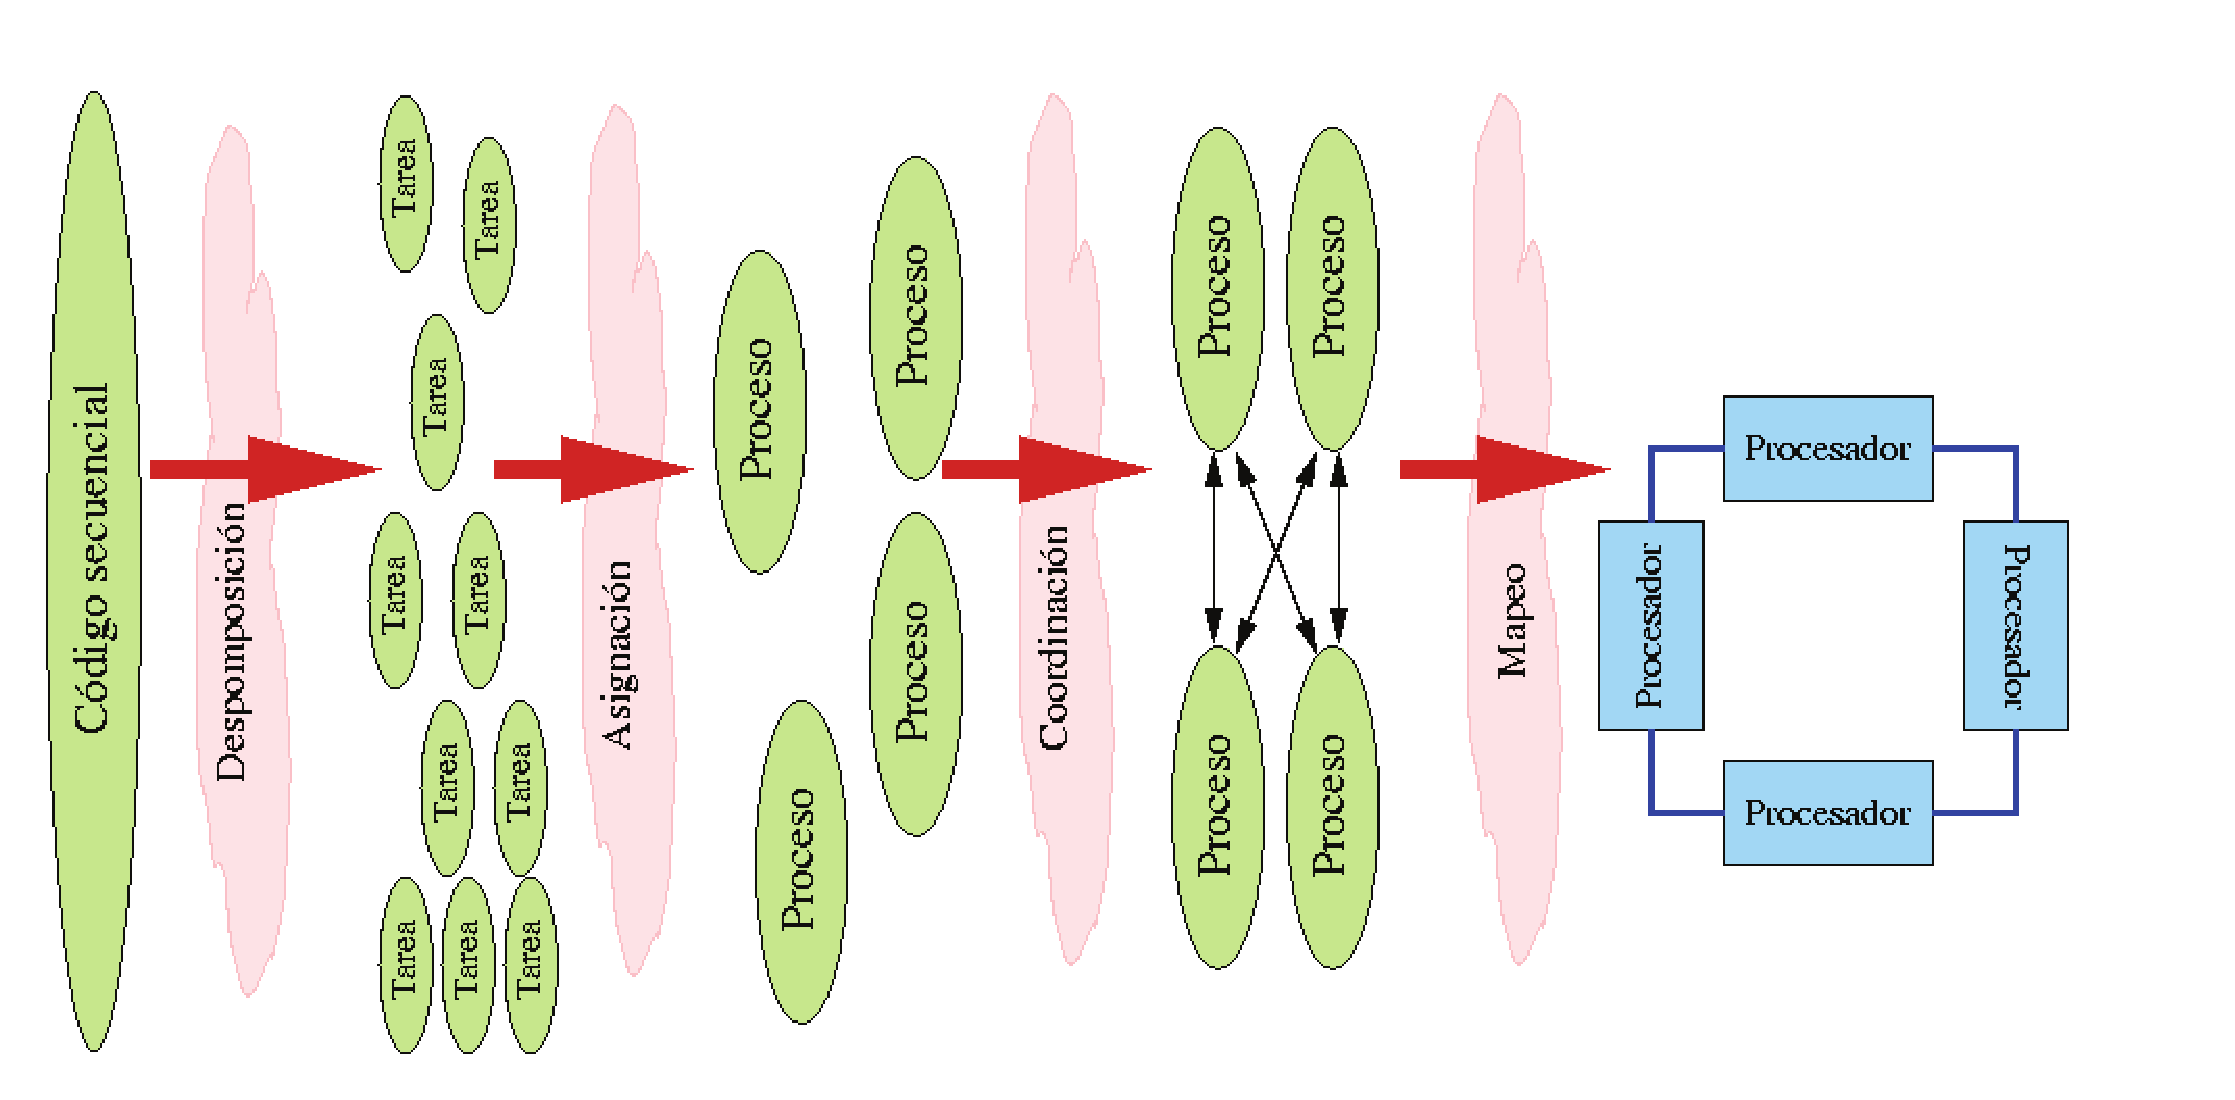
\includegraphics[scale=0.3]{../figuras/figura01.eps} 
\caption{Una figura grande}
\end{figure}
\end{frame}
\end{comment}

\end{document}

